\section{Experimental Results}
\label{experiment}

\subsection{Dataset}
\label{experiment:dataset}
We experiment on trajectories data in four cities from \cite{ijcai15} that were
extracted from Yahoo! Flickr Creative Commons 100M (a.k.a. YFCC100M) dataset\cite{yfcc100m},
and trajectories data in Melbourne that was extracted from YFCC100M the same way described in \cite{ht10, ijcai15},
dataset statistics are available in table \ref{table:data:all}-\ref{table:data:nofew}.

An example of trajectory in Melbourne was shown in figure \ref{fig:traj}.

\begin{figure}
\centering
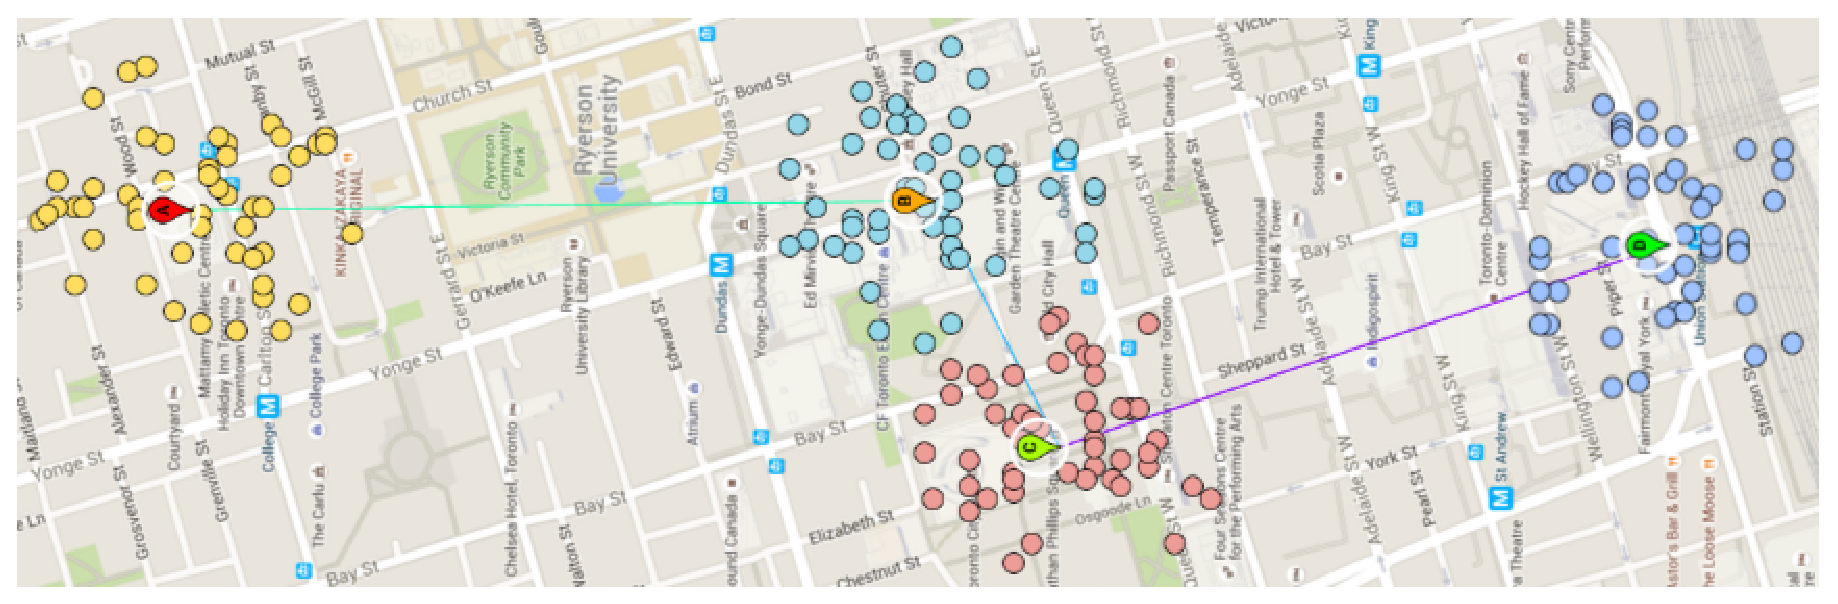
\epsfig{file=traj_eg.eps, width=3.5in}
\caption{An example of trajectory}
\label{fig:traj}
\end{figure}

\subsection{Dataset preprocess}
\label{experiment:datapreprocess}
Trajectories in all datasets are preprocessed such that no self-loops and sub-tours exist.
Concretely, after splitting a sequence of photos by a given time gap and mapping photos to a set of POIs\cite{ht10, ijcai15},
a trajectory was extracted from the result POI visiting sequence such that the order of POIs in the trajectory is the same as 
the order of the first occurrence of POIs in the visiting sequence.


\begin{table*}
\centering
\caption{Datasets description}
\label{table:data:all}
\begin{tabular}{lrrrrr} \hline
\textbf{Dataset} & \textbf{\#Photos} & \textbf{\#POI Visits} & \textbf{\#Trajectories} & \textbf{\#Users} \\ \hline
Edinburgh & 82,060 & 33,944 & 5,028 & 1,454 \\ 
Glasgow & 29,019 & 11,434 & 2,227 & 601 \\ 
Osaka & 392,420 & 7,747 & 1,115 & 450 \\ 
Toronto & 157,505 & 39,419 & 6,057 & 1,395 \\ 
\hline
\end{tabular}
\end{table*}



\subsection{Evaluation Metrics}
\label{experiment:metric}
We use leave-one-out cross validation to evaluate different trajectory recommendation algorithms,
i.e., when evaluating a specific trajectory of a user, all other trajectories of this user as well as 
all trajectories of other users to train the recommendation algorithm.
Then employ trajectory F1-score defined in \cite{ijcai15} to compare the performance of different algorithms.


\subsection{Comparison}
% the way to binning POI features, #clusters of POIs,
\label{experiment:comparison}

We compared the experimental results on trajectory datasets between the proposed methods and other 7 methods:
\begin{itemize}
\item Random: choose POIs uniformly at random (without replacement) from the set of POIs $\mathcal{P} \setminus \{p_s, p_e \}$ to visit.
\item PersTour-T.5\cite{ijcai15}: personalised trajectory recommendation method described in \cite{ijcai15}, 
      time-based user interest was used and $\eta = 0.5$.
\item PersTour-T1\cite{ijcai15}: the same as PersTour-T.5, but set $\eta=1.0$.
\item PersTour-L.5: PersTour\cite{ijcai15} with budget constraint replaced with the number POIs to visit, i.e., $L$,
      similar to PersTour, we use time-based user interest and set $\eta$ to $0.5$.
\item PersTour-L1: the same as PersTour-L.5, but set $\eta=1.0$.
\item RankP: choose POIs according to the ranking based on POI popularity.
\item RankF: choose POIs according to the ranking based on POI features described in section \ref{method:ranking}.
\item MC-DP: recommend trajectory according to the Markov Chain with transition matrix described in section \ref{method:transition},
      use Viterbi algorithm to compute the most likely trajectory w.r.t. constraints $(p_s, p_e, L)$.
\item MC-ILP: the same as MC-DP, but use integer linear programming to compute the most likely trajectory.
\item Prop-DP: one of the proposed methods, combining POI ranking based on features 
      described in section \ref{method:ranking} and the Markov Chain with transition matrix described in section \ref{method:transition},
      use dynamic programming to compute the most likely trajectory w.r.t. constraints $(p_s, p_e, L)$.
\item Prop-ILP: the second proposed method, same as Prop-DP,
      but use integer linear programming to compute the most likely trajectory.
\item CRF: structured prediction using ChainCRF with OneSlackSSVM to recommend trajectory.
\item CRF1: structured prediction using EdgeFeatureGraphCRF with OneSlackSSVM to recommend trajectory.
\end{itemize}

The regularisation parameter of rankSVM in RankF, Prop-DP and Prop-ILP was set to $1000$, and $1$ for CRF and CRF1,
$\alpha=\beta=0.5$ in Prop-DP, Prop-ILP, 
$K=100$ for user specific setting in RankF, RankP, MC-DP, MC-ILP, Prop-DP and Prop-ILP,
POI features used in MC-DP, MC-ILP, Prop-DP and Prop-ILP were discretized using $5$ bins or clusters.


%\begin{tabular}{c|ccccccc|cccccccc} \hline
%\multirow{2}{*}{Dataset} & \multicolumn{7}{|c|}{User agnostic} & \multicolumn{8}{|c}{User specific} \\ \cline{2-15}
%                         & Rand & RankP & RankF & MC-DP & MC-ILP & Pro-DP & Pro-ILP 
%                         & PersTour & PersTour-L & RankP & RankF & MC-DP & MC-ILP & Pro-DP & Pro-ILP \\ \hline
%Toronto           & $1\pm0$ & $1\pm0$ & $1\pm0$ & $1\pm0$ & $1\pm0$ & $1\pm0$ & $1\pm0$ 
%                  & $1\pm0$ & $1\pm0$ & $1\pm0$ & $1\pm0$ & $1\pm0$ & $1\pm0$ & $\mathbf{1\pm0}$ & $1\pm0$ \\


\begin{table*}
\centering
\caption{Performance comparison on four datasets in terms of trajectory F$_1$-score}
\begin{tabular}{l|cccc} \hline
 & Edinburgh & Glasgow & Osaka & Toronto \\ \hline
Random & $0.571\pm0.139$ & $0.632\pm0.124$ & $0.628\pm0.114$ & $0.621\pm0.128$ \\
PersTour-T.5 & $0.657\pm0.222$ & $0.804\pm0.214$ & $0.709\pm0.224$ & $0.720\pm0.215$ \\
PersTour-T1 & $0.611\pm0.201$ & $0.723\pm0.209$ & $0.642\pm0.186$ & $0.710\pm0.219$ \\
PersTour-L.5 & $0.651\pm0.143$ & $0.662\pm0.102$ & $0.699\pm0.139$ & $0.642\pm0.112$ \\
PersTour-L1 & $0.596\pm0.138$ & $0.642\pm0.113$ & $0.657\pm0.142$ & $0.612\pm0.114$ \\
RankP & $0.701\pm0.160$ & $0.746\pm0.167$ & $0.666\pm0.130$ & $0.679\pm0.120$ \\
RankF & $0.694\pm0.155$ & $0.777\pm0.170$ & $0.690\pm0.108$ & $0.753\pm0.167$ \\
MC-DP & $0.629\pm0.171$ & $0.721\pm0.164$ & $0.690\pm0.160$ & $0.662\pm0.156$ \\
MC-ILP & $0.678\pm0.149$ & $0.738\pm0.169$ & $0.720\pm0.148$ & $0.688\pm0.139$ \\
Prop-DP & $0.647\pm0.173$ & $0.744\pm0.172$ & $0.719\pm0.167$ & $0.691\pm0.171$ \\
Prop-ILP & $0.688\pm0.153$ & $0.764\pm0.172$ & $0.733\pm0.157$ & $0.726\pm0.152$ \\
CRF & $\mathbf{0.847\pm0.159}$ & $\mathbf{0.838\pm0.173}$ & $\mathbf{0.762\pm0.162}$ & $\mathbf{0.879\pm0.154}$ \\
\hline
\end{tabular}
\end{table*}


\begin{table*}
\centering
\caption{Performance comparison on four datasets in terms of $\tau$}
\begin{tabular}{l|cccc} \hline
 & Edinburgh & Glasgow & Osaka & Toronto \\ \hline
Random & $0.260\pm0.156$ & $0.319\pm0.166$ & $0.313\pm0.145$ & $0.309\pm0.166$ \\
PersTour-L.5 & $0.351\pm0.206$ & $0.351\pm0.162$ & $0.426\pm0.247$ & $0.329\pm0.158$ \\
PersTour-L1 & $0.289\pm0.174$ & $0.332\pm0.159$ & $0.365\pm0.224$ & $0.292\pm0.134$ \\
RankP & $0.421\pm0.257$ & $0.504\pm0.297$ & $0.367\pm0.198$ & $0.378\pm0.203$ \\
RankF & $0.409\pm0.243$ & $0.559\pm0.307$ & $0.385\pm0.185$ & $0.508\pm0.297$ \\
MC-DP & $0.404\pm0.229$ & $0.482\pm0.285$ & $0.458\pm0.261$ & $0.404\pm0.229$ \\
MC-ILP & $0.390\pm0.235$ & $0.488\pm0.296$ & $0.463\pm0.267$ & $0.399\pm0.233$ \\
Prop-DP & $0.420\pm0.243$ & $0.535\pm0.298$ & $0.515\pm0.276$ & $0.451\pm0.264$ \\
Prop-ILP & $0.401\pm0.245$ & $0.535\pm0.309$ & $0.489\pm0.287$ & $0.459\pm0.269$ \\
CRF & $\mathbf{0.721\pm0.289}$ & $\mathbf{0.705\pm0.310}$ & $\mathbf{0.540\pm0.306}$ & $\mathbf{0.774\pm0.292}$ \\
\hline
\end{tabular}
\end{table*}


\subsection{Analysis of Experimental Results}
\label{experiment:analysis}
